% Digital Logic Report Template
% Created: 2020-02-13 Sebastian Lopez, Megan Gordon, and Jane Ross  

%==========================================================
%=========== Document Setup  ==============================

% Formatting defined by class file
\documentclass[11pt]{article}

% ---- Document formatting ----
\usepackage[margin=1in]{geometry}	% Narrower margins
\usepackage{booktabs}				% Nice formatting of tables
\usepackage{graphicx}				% Ability to include graphics

%\setlength\parindent{0pt}	% Do not indent first line of paragraphs 
\usepackage[parfill]{parskip}		% Line space b/w paragraphs
%	parfill option prevents last line of pgrph from being fully justified

% Parskip package adds too much space around titles, fix with this
\RequirePackage{titlesec}
\titlespacing\section{0pt}{8pt plus 4pt minus 2pt}{3pt plus 2pt minus 2pt}
\titlespacing\subsection{0pt}{4pt plus 4pt minus 2pt}{-2pt plus 2pt minus 2pt}
\titlespacing\subsubsection{0pt}{2pt plus 4pt minus 2pt}{-6pt plus 2pt minus 2pt}

% ---- Hyperlinks ----
\usepackage[colorlinks=true,urlcolor=blue]{hyperref}	% For URL's. Automatically links internal references.

% ---- Code listings ----
\usepackage{listings} 					% Nice code layout and inclusion
\usepackage[usenames,dvipsnames]{xcolor}	% Colors (needs to be defined before using colors)

% Define custom colors for listings
\definecolor{listinggray}{gray}{0.98}		% Listings background color
\definecolor{rulegray}{gray}{0.7}			% Listings rule/frame color

% Style for Verilog
\lstdefinestyle{Verilog}{
	language=Verilog,					% Verilog
	backgroundcolor=\color{listinggray},	% light gray background
	rulecolor=\color{blue}, 			% blue frame lines
	frame=tb,							% lines above & below
	linewidth=\columnwidth, 			% set line width
	basicstyle=\small\ttfamily,	% basic font style that is used for the code	
	breaklines=true, 					% allow breaking across columns/pages
	tabsize=3,							% set tab size
	commentstyle=\color{gray},	% comments in italic 
	stringstyle=\upshape,				% strings are printed in normal font
	showspaces=false,					% don't underscore spaces
}

% How to use: \Verilog[listing_options]{file}
\newcommand{\Verilog}[2][]{%
	\lstinputlisting[style=Verilog,#1]{#2}
}




%======================================================
%=========== Body  ====================================
\begin{document}

\title{ELC 2137 Lab \#5: Intro to Verilog }
\author{Sebastian Lopez, Megan Gordon, and Jane Ross }

\maketitle


\section*{Summary}

In this lab we organized the files and adhered to the given folder structure. We had to learn the basic Verilog syntax and used it to create simple components and systems. We then created a full adder using both gate-level and functional/behavioral styles of coding. Following that we combined full adder components to create a 2-bit and 4-bit adder/subtractor. Throughout the process of the lab we also had to create test benches in order verify our designs.  

\section*{Q\&A}


\begin{enumerate}
	\item \textbf{Comment on whether the simulations match the expected output values.} 
		
	In last week's lab we found the expected output values using variables a, b, and mode. This week after testing and running the code, our simulations did match the results of the expected outcome.  
	
	\item \textbf{What is the one thing you still don't understand about Verilog?}
	
	We don't fully understand the conditions of the if statements. We are also not fully understanding the application of a proper 'always' statement. 
	 
\end{enumerate}

\section*{Results}


\begin{enumerate}
	\item All of the Verilog Code 
	
\begin{lstlisting}[style=Verilog,
caption=Half-adder Source Code,
label=halfadder:ex
]
`timescale 1ns / 1ps
// Sebastian Lopez, Megan Gordon , Jane Ross ELC 2137, 2020-02-19


module halfadder (input a1, b1,
output c1, s1);

xor(s1, a1, b1);
and(c1, a1, b1);


endmodule //halfadder
\end{lstlisting}

\begin{lstlisting}[style=Verilog,
caption=Half-adder Test Bench Code,
label=halfadder_test:ex
]
`timescale 1ns / 1ps
// Sebastian Lopez, Megan Gordon , Jane Ross  ELC 2137, 2020-02-19


module halfadder_test ();

reg a1_in, b1_in; 
wire c1_out, s1_out;

halfadder ha0(
.a1(a1_in), .b1(b1_in), 
.c1(c1_out), .s1(s1_out));

initial
begin
a1_in = 0;
b1_in = 0;
#10;

//Test Case #2
a1_in = 0;
b1_in = 1;
#10
$finish;
end

endmodule //halfadder_test  
\end{lstlisting}

\begin{lstlisting}[style=Verilog,
caption=Full-adder Source Code,
label=fulladder:ex
]
`timescale 1ns / 1ps
// Jane Ross, Megan Gordon and Sebastian Lopez ELC 2137, 2020-02-19

module fulladder(
input a1_in, b1_in, cin,
output s2,cout, c2
);

wire s1, c1, c2;

xor(cout, c1, c2);

halfadder ha1(
.a1(a1_in), .b1(b1_in), 
.c1(c1), .s1(s1)); 
halfadder ha2(
.a1(s1), .b1(cin), 
.c1(c2), .s1(s2));
endmodule//fulladder

\end{lstlisting}

\begin{lstlisting}[style=Verilog,
caption=Full-adder Test Bench Code,
label=fulladder_test:ex
]
`timescale 1ns / 1ps
// Sebastian Lopez, Megan Gordon , Jane Ross ELC 2137, 2020-02-19

module fulladder_test();
reg a1_in, b1_in, cin;
wire s1, c1, c2, s2, cout;

halfadder ha1(
.a1(a1_in), .b1(b1_in), 
.c1(c1), .s1(s1)); 
halfadder ha2(
.a1(s1), .b1(cin), 
.c1(c2), .s1(s2));

assign cout = c2 ^ c1;


initial
begin
//Test case #1
a1_in = 0;
b1_in = 0;
cin = 0;
#10;


//Test Case #2
a1_in = 1;
b1_in = 0;
cin = 0;
#10

//Test Case #3
a1_in = 1;
b1_in = 1;
cin = 0;
#10

//Test case #4
a1_in = 0;
b1_in = 0;
cin = 1;
#10

//Test case #5
a1_in = 1;
b1_in = 0;
cin = 1;
#10

//Test case #6
a1_in = 1;
b1_in = 1;
cin = 1;
#10

$finish;
end


endmodule//fulladder_test
\end{lstlisting}

\begin{lstlisting}[style=Verilog,
caption=2-bit adder Source Code,
label=2-bit adder:ex
]
`timescale 1ns / 1ps
// Jane Ross, Megan Gordon and Sebastian Lopez  ELC 2137, 2020-02-19

module addsub(
input [1:0] a1, b1, a2, b2, mode,
output s2,cout2, s4
);

wire x1,x2, c2, c3, s3, c4, x3;

xor(x1,b1,mode); 
xor(x2,b2,mode); 
xor(x3,c4,c3);
xor(cout2,x3,mode); 

fulladder fa1( 
.a1(a1), .x1(x1),
.s2(s2), .c2(c2));

halfadder ha1(
.a2(a2), .x2(x2), 
.s3(s3), .c3(c3)); 
halfadder ha2(
.s3(s3), .c2(c2), 
.s4(s4), .c4(c4));

endmodule//addsub
\end{lstlisting}

\begin{lstlisting}[style=Verilog,
caption=2-bit adder Test Bench Code,
label=2-bit adder_test:ex
]
`timescale 1ns / 1ps
// Jane Ross, Megan Gordon and Sebastian Lopez  ELC 2137, 2020-02-19

module addsub_test();

reg a1, b1, a2, b2, mode;
wire x1,x2, c2, c3, s3, c4, x3, s2,cout2, s4;

fulladder fa1( 
.a1(a1), .x1(x1),
.s2(s2), .c2(c2));

halfadder ha1(
.a2(a2), .x2(x2), 
.s3(s3), .c3(c3)); 
halfadder ha2(
.s3(s3), .c2(c2), 
.s4(s4), .c4(c4));

assign x1 = mode ^ b1; 
assign x2 = mode ^ b2; 
assign x3 = c4 ^ c3; 
assign cout2 = x3 ^ mode; 



initial
begin

//Test #1
a1 = 0;
a2 = 0;
b1 = 1;
b2 = 0;
mode = 1;
#10

//Test #2
a1 = 0;
a2 = 0;
b1 = 0;
b2 = 1;
mode = 1;
#10

//Test #3
a1 = 0;
a2 = 0;
b1 = 1;
b2 = 1;
mode = 1;
#10

//Test #4
a1 = 1;
a2 = 0;
b1 = 1;
b2 = 0;
mode = 1;
#10

//Test #5
a1 = 0;
a2 = 1;
b1 = 1;
b2 = 0;
mode = 1;
#10

//Test #6
a1 = 0;
a2 = 1;
b1 = 0;
b2 = 0;
mode = 1;
#10

$finish;
end

endmodule//addsub_test
\end{lstlisting}

	\item Block-diagrams for each Module 

\begin{figure}[ht]\centering
	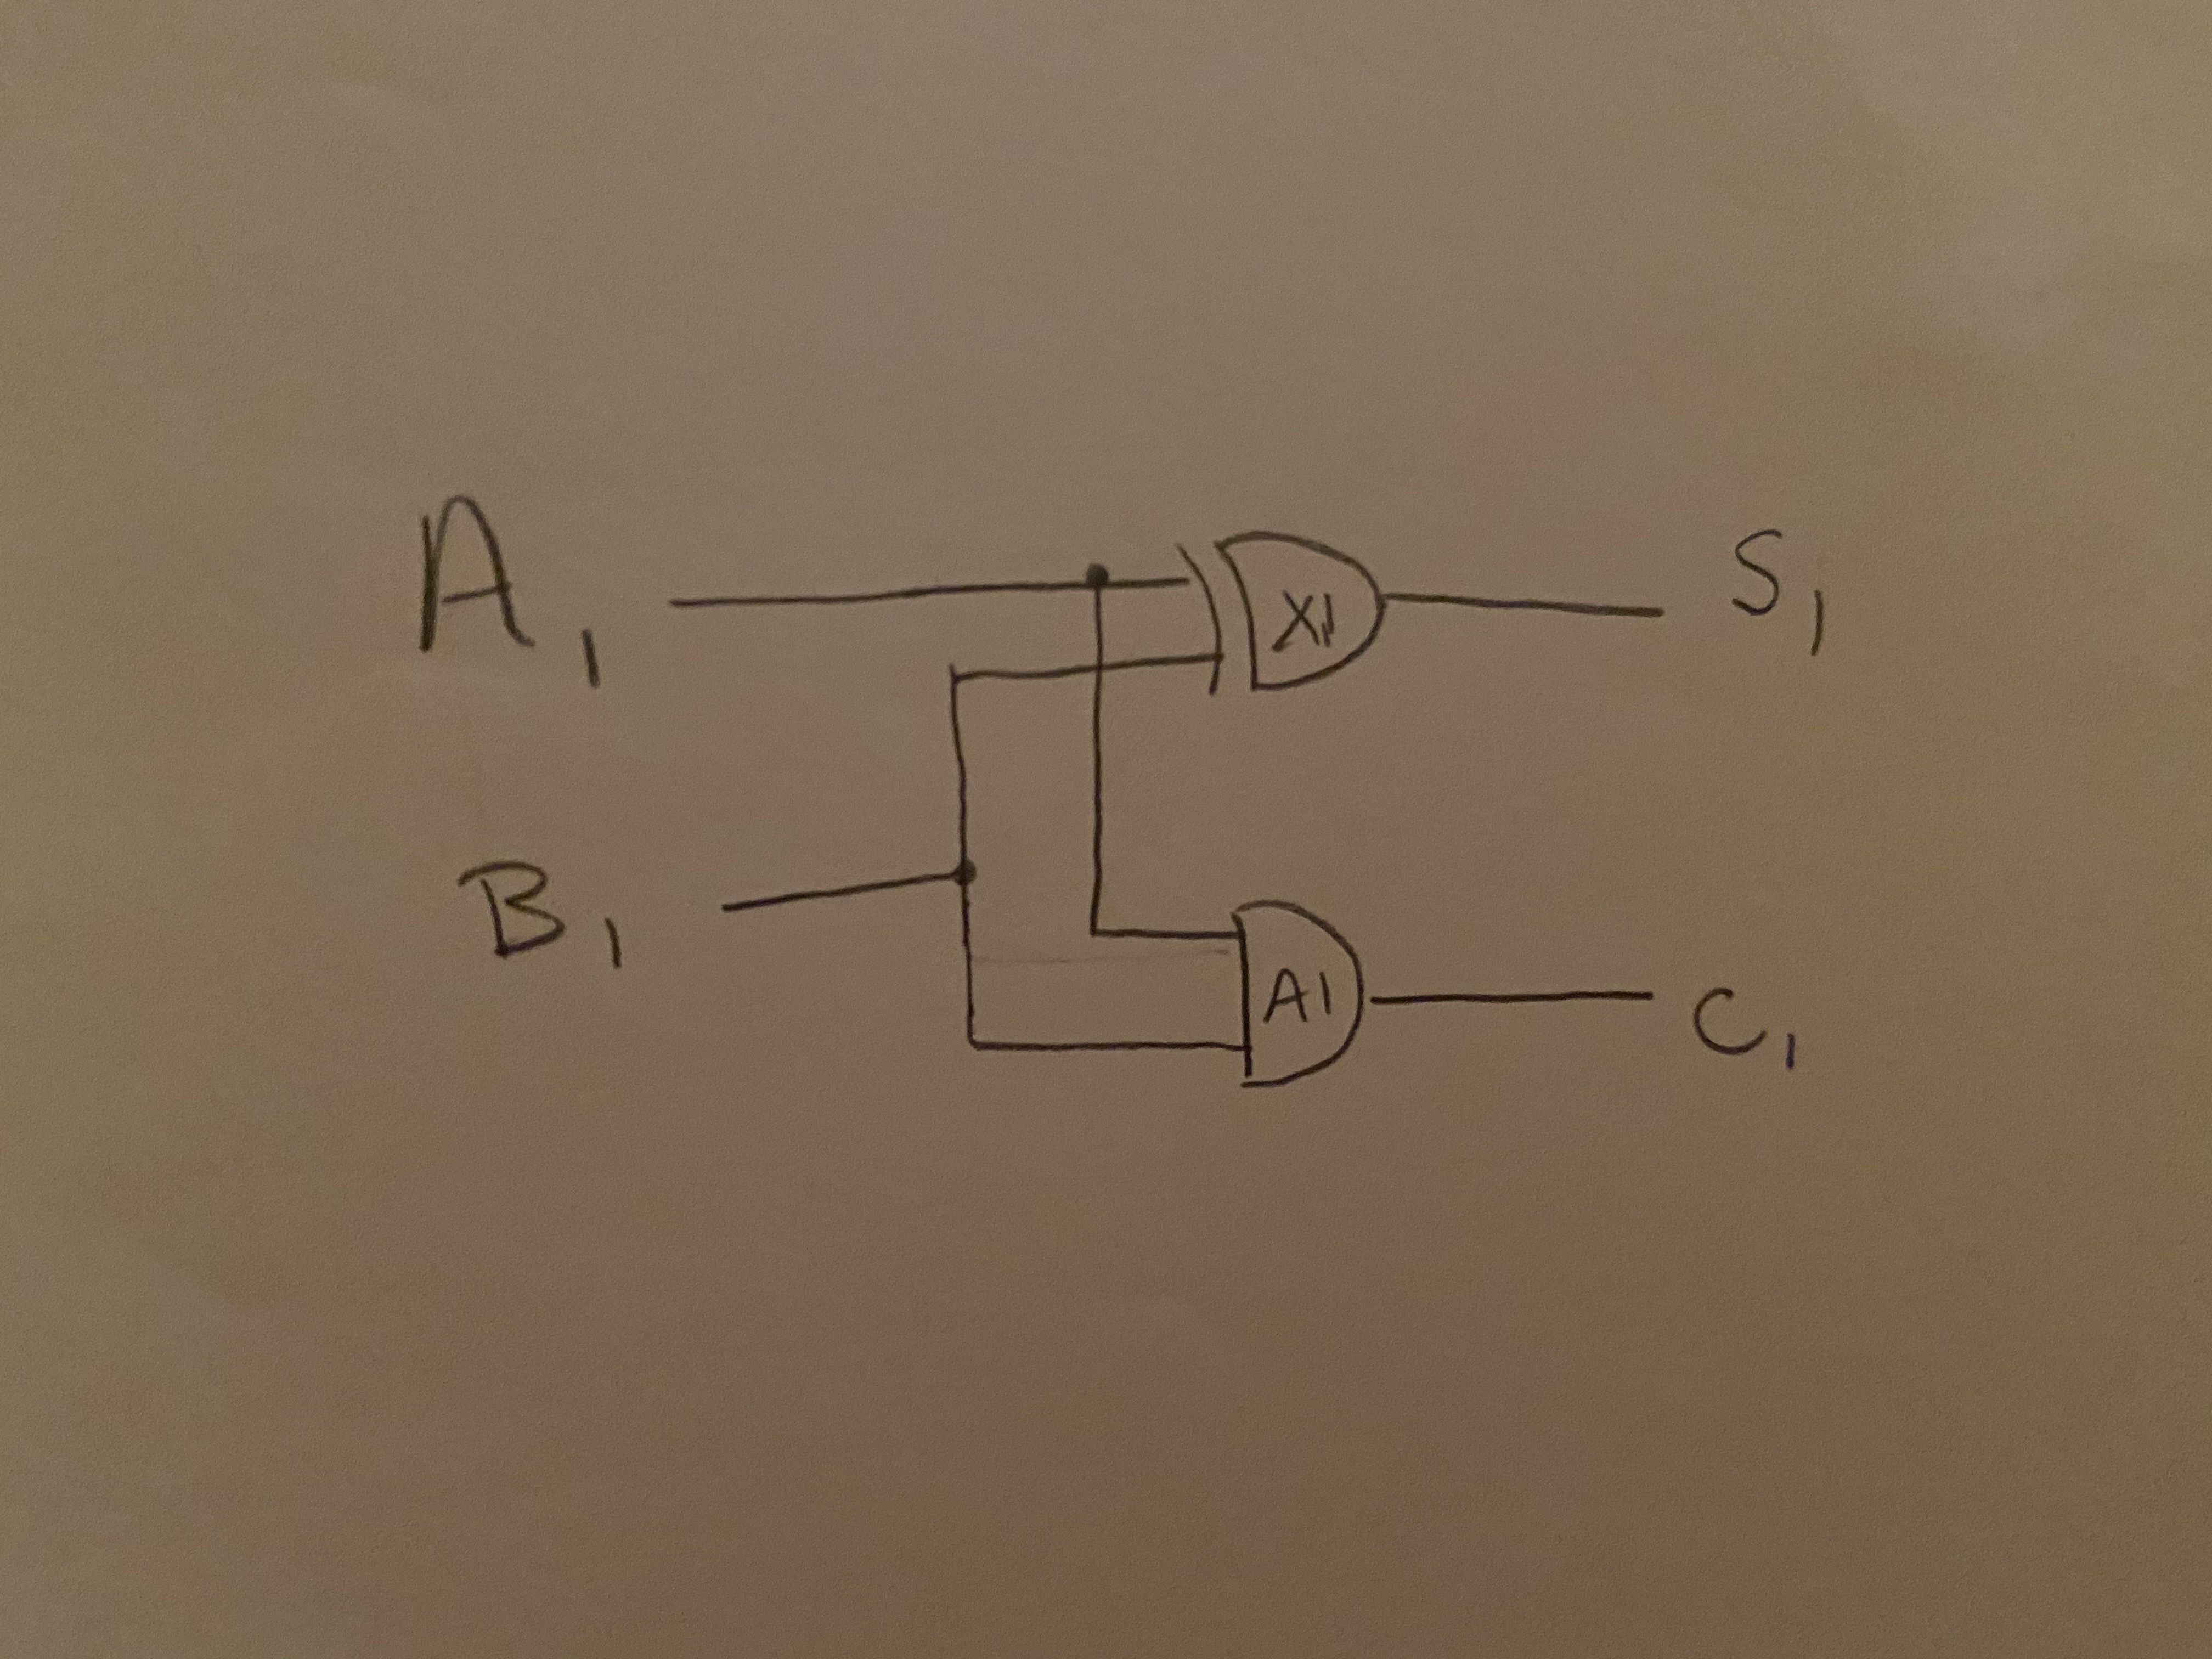
\includegraphics[width=0.6\textwidth, trim=10cm 10cm 10cm 10cm,clip]{Half-Adder Lab05}
	\caption{This is the diagram for the Half Adder}
	\label{fig:Half-Adder}	
\end{figure}

\begin{figure}[ht]\centering
	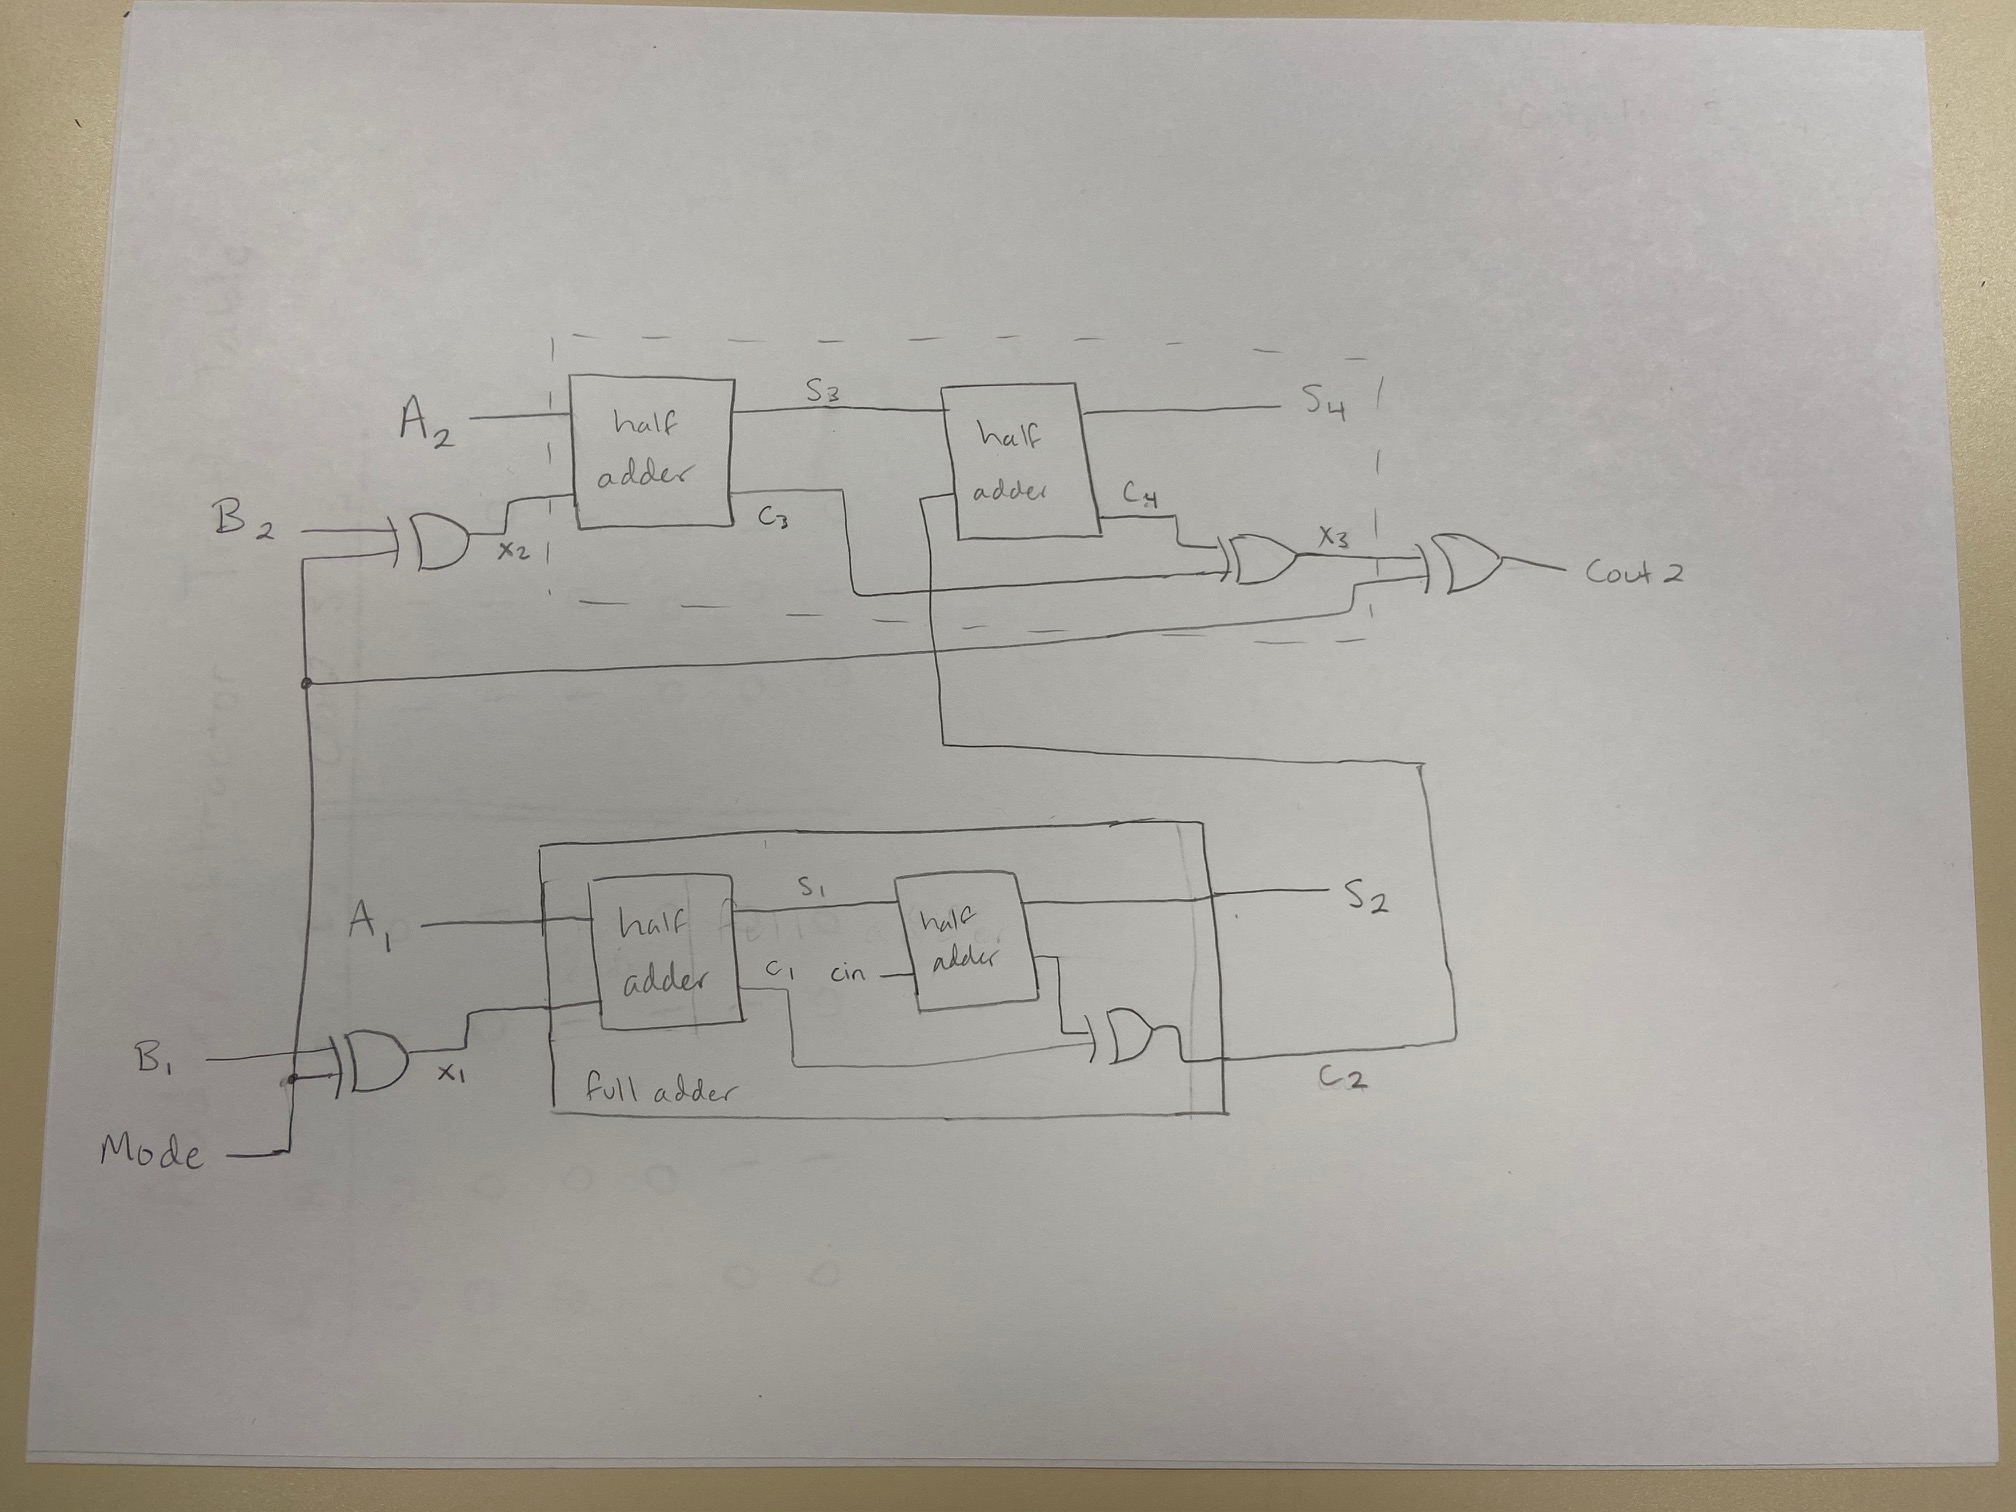
\includegraphics[width=0.6\textwidth, trim=3cm 10cm 10cm 10cm,clip]{2-bit Adder Lab05}
	\caption{This is the diagram for the Full and 2-bit Adder}
	\label{fig:Full_2-bit_Adder}	
\end{figure}

	\item ERTs and screenshots for Behavioral Simulations 
	
\begin{table}[ht]\centering
	\caption{Half Adder ERT}
	\label{tbl:Half_Adder_ERT}
	\begin{tabular}{c||cc|cc}
		\toprule
		Time (ns) & A1 & B1 & C1 & S1\\
		\midrule
		0 & 0 & 1 & 0 & 1\\
		10 & 0 & 0 & 1 & 1\\
		20 & 0 & 0 & 0 & 1\\
		30 & 0 & 1 & 1 & 0\\
		\bottomrule
	\end{tabular} 
\end{table} 

\begin{table}[ht]\centering
	\caption{Full Adder ERT}
	\label{tbl:Half_Adder_ERT}
	\begin{tabular}{c||ccc|cc}
		\toprule
		Time (ns) & A1 & B1 & Cin & Cout & S\\
		\midrule
		0 & 0 & 0 & 0 & 0 & 0\\
		10 & 1 & 0 & 0 & 0 & 1\\
		20 & 1 & 1 & 0 & 1 & 0\\
		30 & 0 & 0 & 1 & 0 & 1\\
		40 & 1 & 0 & 1 & 1 & 0\\
		50 & 1 & 1 & 1 & 1 & 1\\
		\bottomrule
	\end{tabular} 
\end{table} 

\begin{table}[ht]\centering
	\caption{Full Adder ERT}
	\label{tbl:Half_Adder_ERT}
	\begin{tabular}{c||ccccc|ccc}
		\toprule
		Time (ns) & A1 & B1 & A2 & B2 & Mode & Cout & S2 & S4\\
		\midrule
		0 & 0 & 0 & 0 & 0 & 0 & 0 & 0 & 0\\
		10 & 0 & 1 & 0 & 0 & 1 & 1 & 1 & 1\\
		20 & 0 & 0 & 0 & 1 & 1 & 1 & 1 & 0\\
		30 & 0 & 1 & 0 & 1 & 1 & 1 & 0 & 1\\
		40 & 1 & 1 & 0 & 0 & 0 & 0 & 0 & 0\\
		50 & 0 & 1 & 1 & 0 & 0 & 0 & 0 & 1\\
		60 & 0 & 0 & 1 & 0 & 0 & 0 & 1 & 0\\	
		\bottomrule
	\end{tabular} 
\end{table} 

	
\begin{figure}[ht]\centering
	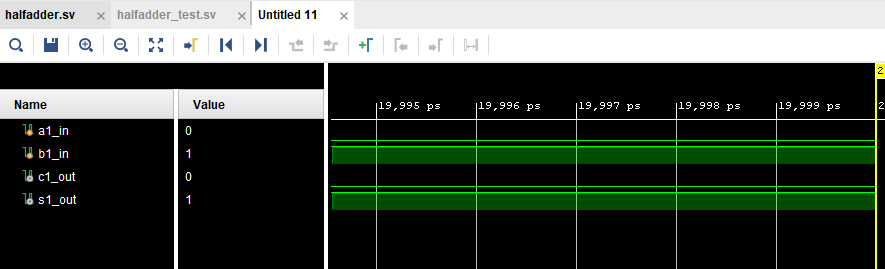
\includegraphics[width=0.75\textwidth]{Half Adder Simulation}
	\caption{This is the Half Adder Simulation Screenshot.}
	\label{fig:half_adder_sim}	
\end{figure}

\begin{figure}[ht]\centering
	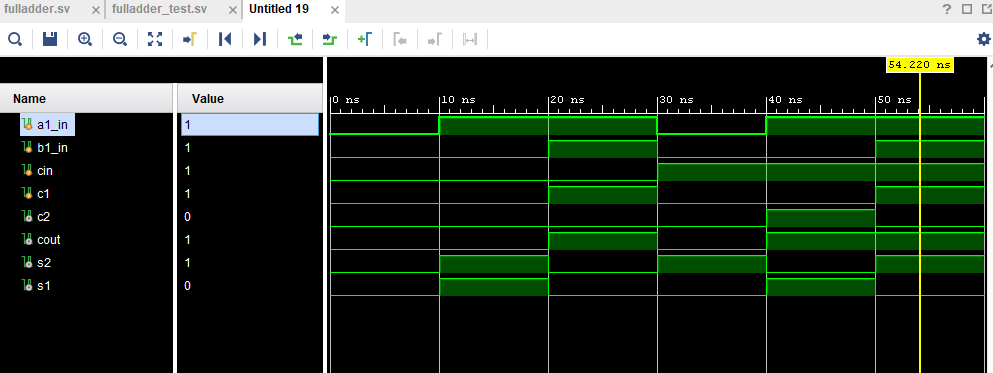
\includegraphics[width=0.75\textwidth]{Full Adder Simulation}
	\caption{This is the Full Adder Simulation Screenshot.}
	\label{fig:full_adder_sim}	
\end{figure}

\end{enumerate}
	
\end{document}	
	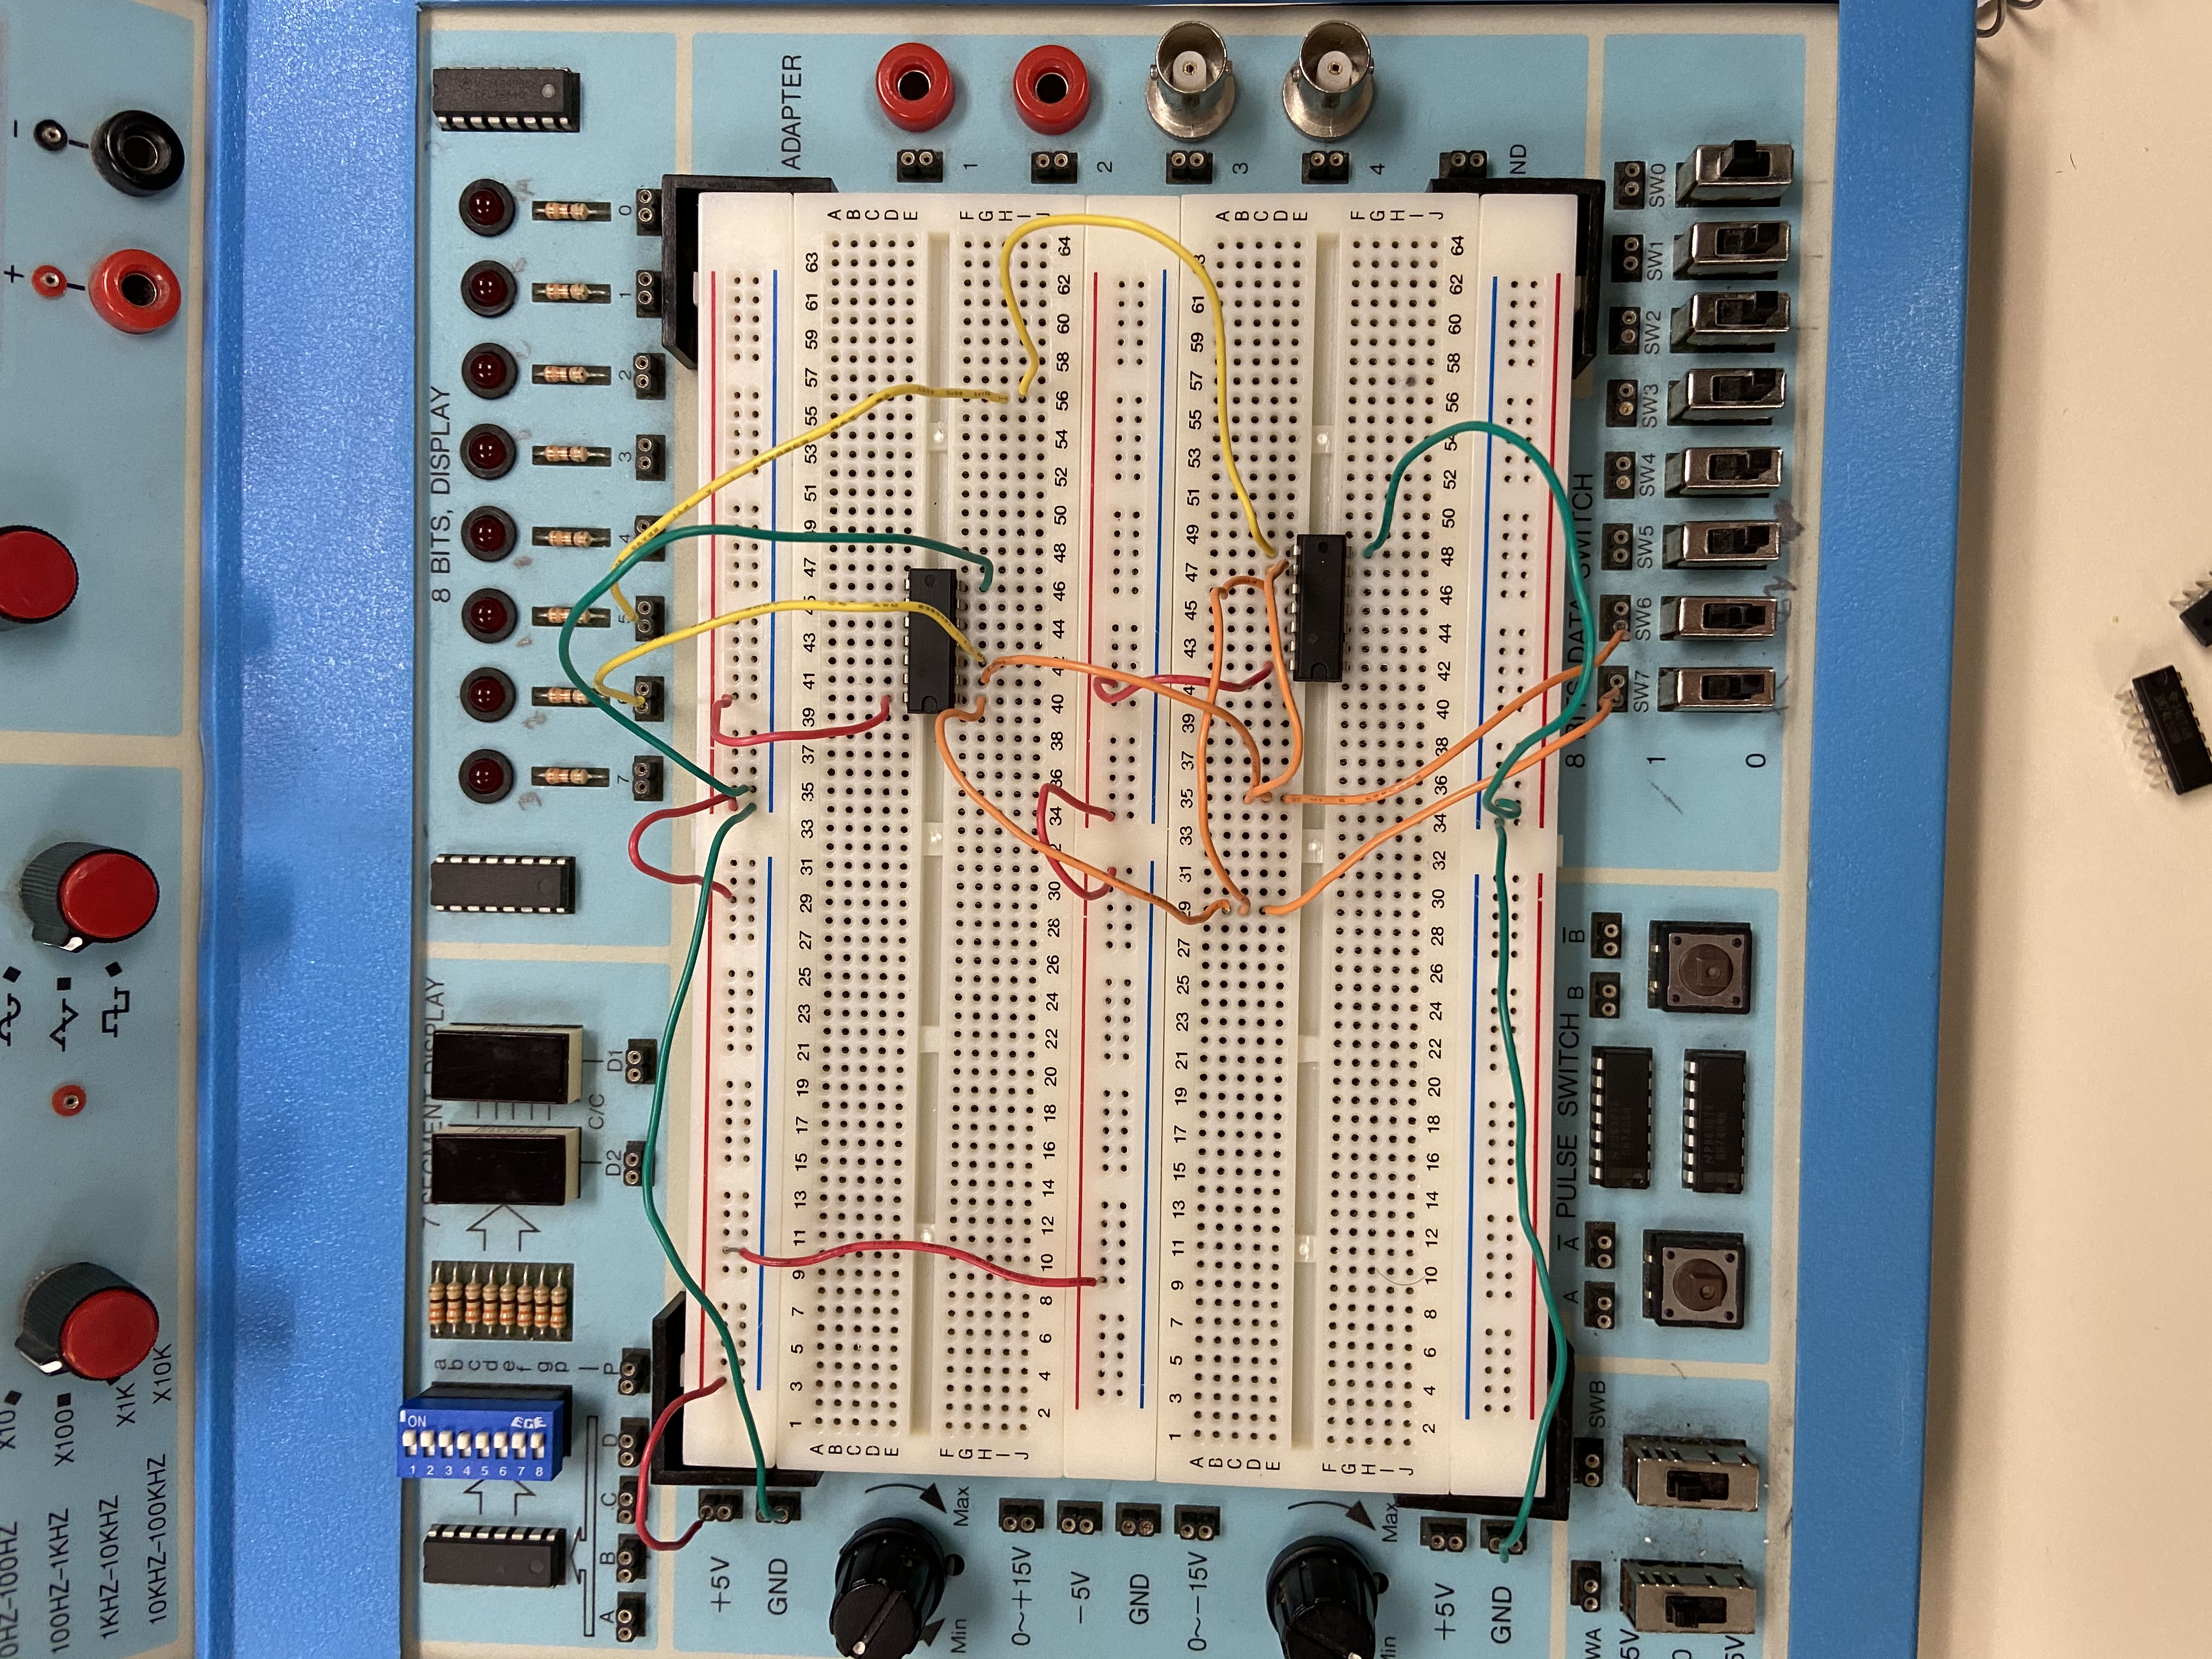
\includegraphics[width=0.75\textwidth]{Half Adder}
	\caption{This is the Half Adder}
	\label{fig:half_adder}	
\end{figure}
	
\end{enumerate}

\end{document}
